\documentclass[twoside]{book}

% Packages required by doxygen
\usepackage{fixltx2e}
\usepackage{calc}
\usepackage{doxygen}
\usepackage[export]{adjustbox} % also loads graphicx
\usepackage{graphicx}
\usepackage[utf8]{inputenc}
\usepackage{makeidx}
\usepackage{multicol}
\usepackage{multirow}
\PassOptionsToPackage{warn}{textcomp}
\usepackage{textcomp}
\usepackage[nointegrals]{wasysym}
\usepackage[table]{xcolor}

% Font selection
\usepackage[T1]{fontenc}
\usepackage[scaled=.90]{helvet}
\usepackage{courier}
\usepackage{amssymb}
\usepackage{sectsty}
\renewcommand{\familydefault}{\sfdefault}
\allsectionsfont{%
  \fontseries{bc}\selectfont%
  \color{darkgray}%
}
\renewcommand{\DoxyLabelFont}{%
  \fontseries{bc}\selectfont%
  \color{darkgray}%
}
\newcommand{\+}{\discretionary{\mbox{\scriptsize$\hookleftarrow$}}{}{}}

% Page & text layout
\usepackage{geometry}
\geometry{%
  a4paper,%
  top=2.5cm,%
  bottom=2.5cm,%
  left=2.5cm,%
  right=2.5cm%
}
\tolerance=750
\hfuzz=15pt
\hbadness=750
\setlength{\emergencystretch}{15pt}
\setlength{\parindent}{0cm}
\setlength{\parskip}{3ex plus 2ex minus 2ex}
\makeatletter
\renewcommand{\paragraph}{%
  \@startsection{paragraph}{4}{0ex}{-1.0ex}{1.0ex}{%
    \normalfont\normalsize\bfseries\SS@parafont%
  }%
}
\renewcommand{\subparagraph}{%
  \@startsection{subparagraph}{5}{0ex}{-1.0ex}{1.0ex}{%
    \normalfont\normalsize\bfseries\SS@subparafont%
  }%
}
\makeatother

% Headers & footers
\usepackage{fancyhdr}
\pagestyle{fancyplain}
\fancyhead[LE]{\fancyplain{}{\bfseries\thepage}}
\fancyhead[CE]{\fancyplain{}{}}
\fancyhead[RE]{\fancyplain{}{\bfseries\leftmark}}
\fancyhead[LO]{\fancyplain{}{\bfseries\rightmark}}
\fancyhead[CO]{\fancyplain{}{}}
\fancyhead[RO]{\fancyplain{}{\bfseries\thepage}}
\fancyfoot[LE]{\fancyplain{}{}}
\fancyfoot[CE]{\fancyplain{}{}}
\fancyfoot[RE]{\fancyplain{}{\bfseries\scriptsize Generated by Doxygen }}
\fancyfoot[LO]{\fancyplain{}{\bfseries\scriptsize Generated by Doxygen }}
\fancyfoot[CO]{\fancyplain{}{}}
\fancyfoot[RO]{\fancyplain{}{}}
\renewcommand{\footrulewidth}{0.4pt}
\renewcommand{\chaptermark}[1]{%
  \markboth{#1}{}%
}
\renewcommand{\sectionmark}[1]{%
  \markright{\thesection\ #1}%
}

% Indices & bibliography
\usepackage{natbib}
\usepackage[titles]{tocloft}
\setcounter{tocdepth}{3}
\setcounter{secnumdepth}{5}
\makeindex

% Hyperlinks (required, but should be loaded last)
\usepackage{ifpdf}
\ifpdf
  \usepackage[pdftex,pagebackref=true]{hyperref}
\else
  \usepackage[ps2pdf,pagebackref=true]{hyperref}
\fi
\hypersetup{%
  colorlinks=true,%
  linkcolor=blue,%
  citecolor=blue,%
  unicode%
}

% Custom commands
\newcommand{\clearemptydoublepage}{%
  \newpage{\pagestyle{empty}\cleardoublepage}%
}

\usepackage{caption}
\captionsetup{labelsep=space,justification=centering,font={bf},singlelinecheck=off,skip=4pt,position=top}

%===== C O N T E N T S =====

\begin{document}

% Titlepage & ToC
\hypersetup{pageanchor=false,
             bookmarksnumbered=true,
             pdfencoding=unicode
            }
\pagenumbering{alph}
\begin{titlepage}
\vspace*{7cm}
\begin{center}%
{\Large Assignment -\/ 1 }\\
\vspace*{1cm}
{\large Generated by Doxygen 1.8.13}\\
\end{center}
\end{titlepage}
\clearemptydoublepage
\pagenumbering{roman}
\tableofcontents
\clearemptydoublepage
\pagenumbering{arabic}
\hypersetup{pageanchor=true}

%--- Begin generated contents ---
\chapter{Class Index}
\section{Class List}
Here are the classes, structs, unions and interfaces with brief descriptions\+:\begin{DoxyCompactList}
\item\contentsline{section}{\hyperlink{classcircle}{circle} }{\pageref{classcircle}}{}
\item\contentsline{section}{\hyperlink{structextreme}{extreme} }{\pageref{structextreme}}{}
\item\contentsline{section}{\hyperlink{classline}{line} }{\pageref{classline}}{}
\item\contentsline{section}{\hyperlink{structnode}{node} }{\pageref{structnode}}{}
\item\contentsline{section}{\hyperlink{classtree}{tree} }{\pageref{classtree}}{}
\end{DoxyCompactList}

\chapter{File Index}
\section{File List}
Here is a list of all files with brief descriptions\+:\begin{DoxyCompactList}
\item\contentsline{section}{Computer\+Graphics\+Project/\+Computer\+Graphics\+Project/\hyperlink{_circle_8cpp}{Circle.\+cpp} }{\pageref{_circle_8cpp}}{}
\item\contentsline{section}{Computer\+Graphics\+Project/\+Computer\+Graphics\+Project/\hyperlink{_circle_8h}{Circle.\+h} }{\pageref{_circle_8h}}{}
\item\contentsline{section}{Computer\+Graphics\+Project/\+Computer\+Graphics\+Project/\hyperlink{_line_8cpp}{Line.\+cpp} }{\pageref{_line_8cpp}}{}
\item\contentsline{section}{Computer\+Graphics\+Project/\+Computer\+Graphics\+Project/\hyperlink{_line_8h}{Line.\+h} }{\pageref{_line_8h}}{}
\item\contentsline{section}{Computer\+Graphics\+Project/\+Computer\+Graphics\+Project/\hyperlink{main_8cpp}{main.\+cpp} }{\pageref{main_8cpp}}{}
\item\contentsline{section}{Computer\+Graphics\+Project/\+Computer\+Graphics\+Project/\hyperlink{tree_8cpp}{tree.\+cpp} }{\pageref{tree_8cpp}}{}
\item\contentsline{section}{Computer\+Graphics\+Project/\+Computer\+Graphics\+Project/\hyperlink{tree_8h}{tree.\+h} }{\pageref{tree_8h}}{}
\end{DoxyCompactList}

\chapter{Class Documentation}
\hypertarget{classcircle}{}\section{circle Class Reference}
\label{classcircle}\index{circle@{circle}}


{\ttfamily \#include $<$Circle.\+h$>$}

\subsection*{Public Member Functions}
\begin{DoxyCompactItemize}
\item 
\hyperlink{classcircle_a05447431f708a932321cf140f36e45be}{circle} (int \hyperlink{classcircle_acb3d4e48483b2ea9837fa75cc0977c0d}{center\+\_\+x}, int \hyperlink{classcircle_ae297efc5c3c3b7a2e6595ed74e324c88}{center\+\_\+y}, int \hyperlink{classcircle_a90f36ddf730f3c068125f9533d1cd7a1}{r})
\item 
void \hyperlink{classcircle_ab64f82d19bb3a5318d1b94bf9946b732}{draw} ()
\end{DoxyCompactItemize}
\subsection*{Private Member Functions}
\begin{DoxyCompactItemize}
\item 
void \hyperlink{classcircle_a2a17a7069348f990b854b7e6d7cef358}{plot\+\_\+circle} (int x, int y, int cx, int cy, int \hyperlink{classcircle_a90f36ddf730f3c068125f9533d1cd7a1}{r}=0, int g=0, int b=0)
\end{DoxyCompactItemize}
\subsection*{Private Attributes}
\begin{DoxyCompactItemize}
\item 
int \hyperlink{classcircle_acb3d4e48483b2ea9837fa75cc0977c0d}{center\+\_\+x}
\item 
int \hyperlink{classcircle_ae297efc5c3c3b7a2e6595ed74e324c88}{center\+\_\+y}
\item 
int \hyperlink{classcircle_a90f36ddf730f3c068125f9533d1cd7a1}{r}
\end{DoxyCompactItemize}


\subsection{Constructor \& Destructor Documentation}
\mbox{\Hypertarget{classcircle_a05447431f708a932321cf140f36e45be}\label{classcircle_a05447431f708a932321cf140f36e45be}} 
\index{circle@{circle}!circle@{circle}}
\index{circle@{circle}!circle@{circle}}
\subsubsection{\texorpdfstring{circle()}{circle()}}
{\footnotesize\ttfamily circle\+::circle (\begin{DoxyParamCaption}\item[{int}]{center\+\_\+x,  }\item[{int}]{center\+\_\+y,  }\item[{int}]{r }\end{DoxyParamCaption})}



\subsection{Member Function Documentation}
\mbox{\Hypertarget{classcircle_ab64f82d19bb3a5318d1b94bf9946b732}\label{classcircle_ab64f82d19bb3a5318d1b94bf9946b732}} 
\index{circle@{circle}!draw@{draw}}
\index{draw@{draw}!circle@{circle}}
\subsubsection{\texorpdfstring{draw()}{draw()}}
{\footnotesize\ttfamily void circle\+::draw (\begin{DoxyParamCaption}{ }\end{DoxyParamCaption})}

\mbox{\Hypertarget{classcircle_a2a17a7069348f990b854b7e6d7cef358}\label{classcircle_a2a17a7069348f990b854b7e6d7cef358}} 
\index{circle@{circle}!plot\+\_\+circle@{plot\+\_\+circle}}
\index{plot\+\_\+circle@{plot\+\_\+circle}!circle@{circle}}
\subsubsection{\texorpdfstring{plot\+\_\+circle()}{plot\_circle()}}
{\footnotesize\ttfamily void circle\+::plot\+\_\+circle (\begin{DoxyParamCaption}\item[{int}]{x,  }\item[{int}]{y,  }\item[{int}]{cx,  }\item[{int}]{cy,  }\item[{int}]{r = {\ttfamily 0},  }\item[{int}]{g = {\ttfamily 0},  }\item[{int}]{b = {\ttfamily 0} }\end{DoxyParamCaption})\hspace{0.3cm}{\ttfamily [private]}}



\subsection{Member Data Documentation}
\mbox{\Hypertarget{classcircle_acb3d4e48483b2ea9837fa75cc0977c0d}\label{classcircle_acb3d4e48483b2ea9837fa75cc0977c0d}} 
\index{circle@{circle}!center\+\_\+x@{center\+\_\+x}}
\index{center\+\_\+x@{center\+\_\+x}!circle@{circle}}
\subsubsection{\texorpdfstring{center\+\_\+x}{center\_x}}
{\footnotesize\ttfamily int circle\+::center\+\_\+x\hspace{0.3cm}{\ttfamily [private]}}

\mbox{\Hypertarget{classcircle_ae297efc5c3c3b7a2e6595ed74e324c88}\label{classcircle_ae297efc5c3c3b7a2e6595ed74e324c88}} 
\index{circle@{circle}!center\+\_\+y@{center\+\_\+y}}
\index{center\+\_\+y@{center\+\_\+y}!circle@{circle}}
\subsubsection{\texorpdfstring{center\+\_\+y}{center\_y}}
{\footnotesize\ttfamily int circle\+::center\+\_\+y\hspace{0.3cm}{\ttfamily [private]}}

\mbox{\Hypertarget{classcircle_a90f36ddf730f3c068125f9533d1cd7a1}\label{classcircle_a90f36ddf730f3c068125f9533d1cd7a1}} 
\index{circle@{circle}!r@{r}}
\index{r@{r}!circle@{circle}}
\subsubsection{\texorpdfstring{r}{r}}
{\footnotesize\ttfamily int circle\+::r\hspace{0.3cm}{\ttfamily [private]}}



The documentation for this class was generated from the following files\+:\begin{DoxyCompactItemize}
\item 
Computer\+Graphics\+Project/\+Computer\+Graphics\+Project/\hyperlink{_circle_8h}{Circle.\+h}\item 
Computer\+Graphics\+Project/\+Computer\+Graphics\+Project/\hyperlink{_circle_8cpp}{Circle.\+cpp}\end{DoxyCompactItemize}

\hypertarget{structextreme}{}\section{extreme Struct Reference}
\label{structextreme}\index{extreme@{extreme}}


{\ttfamily \#include $<$tree.\+h$>$}



Collaboration diagram for extreme\+:
\nopagebreak
\begin{figure}[H]
\begin{center}
\leavevmode
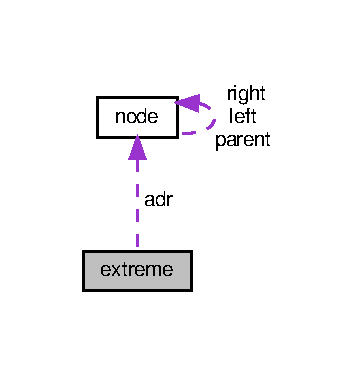
\includegraphics[width=171pt]{structextreme__coll__graph}
\end{center}
\end{figure}
\subsection*{Public Attributes}
\begin{DoxyCompactItemize}
\item 
\hyperlink{structnode}{node} $\ast$ \hyperlink{structextreme_ab6b1591edc7b63297c3499df6c1d869a}{adr}
\item 
int \hyperlink{structextreme_a4a01f7889effe05776f9c7aab111452a}{offset}
\item 
int \hyperlink{structextreme_a80adaa7fa8a2fd6b51e092462628af3e}{level}
\end{DoxyCompactItemize}


\subsection{Member Data Documentation}
\mbox{\Hypertarget{structextreme_ab6b1591edc7b63297c3499df6c1d869a}\label{structextreme_ab6b1591edc7b63297c3499df6c1d869a}} 
\index{extreme@{extreme}!adr@{adr}}
\index{adr@{adr}!extreme@{extreme}}
\subsubsection{\texorpdfstring{adr}{adr}}
{\footnotesize\ttfamily \hyperlink{structnode}{node}$\ast$ extreme\+::adr}

\mbox{\Hypertarget{structextreme_a80adaa7fa8a2fd6b51e092462628af3e}\label{structextreme_a80adaa7fa8a2fd6b51e092462628af3e}} 
\index{extreme@{extreme}!level@{level}}
\index{level@{level}!extreme@{extreme}}
\subsubsection{\texorpdfstring{level}{level}}
{\footnotesize\ttfamily int extreme\+::level}

\mbox{\Hypertarget{structextreme_a4a01f7889effe05776f9c7aab111452a}\label{structextreme_a4a01f7889effe05776f9c7aab111452a}} 
\index{extreme@{extreme}!offset@{offset}}
\index{offset@{offset}!extreme@{extreme}}
\subsubsection{\texorpdfstring{offset}{offset}}
{\footnotesize\ttfamily int extreme\+::offset}



The documentation for this struct was generated from the following file\+:\begin{DoxyCompactItemize}
\item 
Computer\+Graphics\+Project/\+Computer\+Graphics\+Project/\hyperlink{tree_8h}{tree.\+h}\end{DoxyCompactItemize}

\hypertarget{classline}{}\section{line Class Reference}
\label{classline}\index{line@{line}}


{\ttfamily \#include $<$Line.\+h$>$}

\subsection*{Public Member Functions}
\begin{DoxyCompactItemize}
\item 
\hyperlink{classline_a228fedb37c2f7266e833dd2c00ad9fc1}{line} (int \hyperlink{classline_a75af55c0f7d0f1f113d12fd6e1d53ed0}{sx}, int \hyperlink{classline_afd9ace37f8fe42bf6438208f6acfae74}{sy}, int \hyperlink{classline_ab3aa6549e46960b1d65b6286b1e4a5c5}{ex}, int \hyperlink{classline_a9967b1a26c3c8abf1906e5f5e12be9d3}{ey})
\item 
void \hyperlink{classline_ac3edc76a59ee53e240875513073c447c}{draw} ()
\end{DoxyCompactItemize}
\subsection*{Private Attributes}
\begin{DoxyCompactItemize}
\item 
int \hyperlink{classline_a75af55c0f7d0f1f113d12fd6e1d53ed0}{sx}
\item 
int \hyperlink{classline_afd9ace37f8fe42bf6438208f6acfae74}{sy}
\item 
int \hyperlink{classline_ab3aa6549e46960b1d65b6286b1e4a5c5}{ex}
\item 
int \hyperlink{classline_a9967b1a26c3c8abf1906e5f5e12be9d3}{ey}
\end{DoxyCompactItemize}


\subsection{Constructor \& Destructor Documentation}
\mbox{\Hypertarget{classline_a228fedb37c2f7266e833dd2c00ad9fc1}\label{classline_a228fedb37c2f7266e833dd2c00ad9fc1}} 
\index{line@{line}!line@{line}}
\index{line@{line}!line@{line}}
\subsubsection{\texorpdfstring{line()}{line()}}
{\footnotesize\ttfamily line\+::line (\begin{DoxyParamCaption}\item[{int}]{sx,  }\item[{int}]{sy,  }\item[{int}]{ex,  }\item[{int}]{ey }\end{DoxyParamCaption})}



\subsection{Member Function Documentation}
\mbox{\Hypertarget{classline_ac3edc76a59ee53e240875513073c447c}\label{classline_ac3edc76a59ee53e240875513073c447c}} 
\index{line@{line}!draw@{draw}}
\index{draw@{draw}!line@{line}}
\subsubsection{\texorpdfstring{draw()}{draw()}}
{\footnotesize\ttfamily void line\+::draw (\begin{DoxyParamCaption}{ }\end{DoxyParamCaption})}



\subsection{Member Data Documentation}
\mbox{\Hypertarget{classline_ab3aa6549e46960b1d65b6286b1e4a5c5}\label{classline_ab3aa6549e46960b1d65b6286b1e4a5c5}} 
\index{line@{line}!ex@{ex}}
\index{ex@{ex}!line@{line}}
\subsubsection{\texorpdfstring{ex}{ex}}
{\footnotesize\ttfamily int line\+::ex\hspace{0.3cm}{\ttfamily [private]}}

\mbox{\Hypertarget{classline_a9967b1a26c3c8abf1906e5f5e12be9d3}\label{classline_a9967b1a26c3c8abf1906e5f5e12be9d3}} 
\index{line@{line}!ey@{ey}}
\index{ey@{ey}!line@{line}}
\subsubsection{\texorpdfstring{ey}{ey}}
{\footnotesize\ttfamily int line\+::ey\hspace{0.3cm}{\ttfamily [private]}}

\mbox{\Hypertarget{classline_a75af55c0f7d0f1f113d12fd6e1d53ed0}\label{classline_a75af55c0f7d0f1f113d12fd6e1d53ed0}} 
\index{line@{line}!sx@{sx}}
\index{sx@{sx}!line@{line}}
\subsubsection{\texorpdfstring{sx}{sx}}
{\footnotesize\ttfamily int line\+::sx\hspace{0.3cm}{\ttfamily [private]}}

\mbox{\Hypertarget{classline_afd9ace37f8fe42bf6438208f6acfae74}\label{classline_afd9ace37f8fe42bf6438208f6acfae74}} 
\index{line@{line}!sy@{sy}}
\index{sy@{sy}!line@{line}}
\subsubsection{\texorpdfstring{sy}{sy}}
{\footnotesize\ttfamily int line\+::sy\hspace{0.3cm}{\ttfamily [private]}}



The documentation for this class was generated from the following files\+:\begin{DoxyCompactItemize}
\item 
Computer\+Graphics\+Project/\+Computer\+Graphics\+Project/\hyperlink{_line_8h}{Line.\+h}\item 
Computer\+Graphics\+Project/\+Computer\+Graphics\+Project/\hyperlink{_line_8cpp}{Line.\+cpp}\end{DoxyCompactItemize}

\hypertarget{structnode}{}\section{node Struct Reference}
\label{structnode}\index{node@{node}}


{\ttfamily \#include $<$tree.\+h$>$}



Collaboration diagram for node\+:
\nopagebreak
\begin{figure}[H]
\begin{center}
\leavevmode
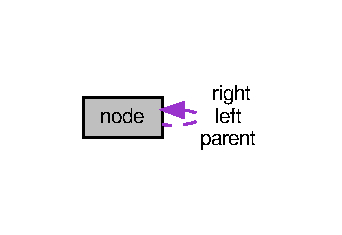
\includegraphics[width=164pt]{structnode__coll__graph}
\end{center}
\end{figure}
\subsection*{Public Attributes}
\begin{DoxyCompactItemize}
\item 
int \hyperlink{structnode_a2d890bb9f6af0ffd73fe79b21124c2a2}{data}
\item 
struct \hyperlink{structnode}{node} $\ast$ \hyperlink{structnode_a3ce38490a651bfda86d88ff955e96abc}{left}
\item 
struct \hyperlink{structnode}{node} $\ast$ \hyperlink{structnode_a875f75abfe22103500535b179828e4e3}{right}
\item 
struct \hyperlink{structnode}{node} $\ast$ \hyperlink{structnode_a05e4fe9e0177ba2d8dbd2c487cfddd53}{parent}
\item 
int \hyperlink{structnode_a3871d43e823ba9542b052912d01709dd}{level}
\item 
int \hyperlink{structnode_a64dd8b65a7d38c632a017d7f36444dbb}{x}
\item 
int \hyperlink{structnode_ae944a3a75efb9856fa5c6f2221e2b49e}{y}
\item 
int \hyperlink{structnode_aeef7855fea382bfb671d7834aefa4b22}{offset}
\item 
bool \hyperlink{structnode_afd9ff5fa3c3ab99d07cac2a7ad9d14a6}{thread}
\end{DoxyCompactItemize}


\subsection{Member Data Documentation}
\mbox{\Hypertarget{structnode_a2d890bb9f6af0ffd73fe79b21124c2a2}\label{structnode_a2d890bb9f6af0ffd73fe79b21124c2a2}} 
\index{node@{node}!data@{data}}
\index{data@{data}!node@{node}}
\subsubsection{\texorpdfstring{data}{data}}
{\footnotesize\ttfamily int node\+::data}

\mbox{\Hypertarget{structnode_a3ce38490a651bfda86d88ff955e96abc}\label{structnode_a3ce38490a651bfda86d88ff955e96abc}} 
\index{node@{node}!left@{left}}
\index{left@{left}!node@{node}}
\subsubsection{\texorpdfstring{left}{left}}
{\footnotesize\ttfamily struct \hyperlink{structnode}{node}$\ast$ node\+::left}

\mbox{\Hypertarget{structnode_a3871d43e823ba9542b052912d01709dd}\label{structnode_a3871d43e823ba9542b052912d01709dd}} 
\index{node@{node}!level@{level}}
\index{level@{level}!node@{node}}
\subsubsection{\texorpdfstring{level}{level}}
{\footnotesize\ttfamily int node\+::level}

\mbox{\Hypertarget{structnode_aeef7855fea382bfb671d7834aefa4b22}\label{structnode_aeef7855fea382bfb671d7834aefa4b22}} 
\index{node@{node}!offset@{offset}}
\index{offset@{offset}!node@{node}}
\subsubsection{\texorpdfstring{offset}{offset}}
{\footnotesize\ttfamily int node\+::offset}

\mbox{\Hypertarget{structnode_a05e4fe9e0177ba2d8dbd2c487cfddd53}\label{structnode_a05e4fe9e0177ba2d8dbd2c487cfddd53}} 
\index{node@{node}!parent@{parent}}
\index{parent@{parent}!node@{node}}
\subsubsection{\texorpdfstring{parent}{parent}}
{\footnotesize\ttfamily struct \hyperlink{structnode}{node}$\ast$ node\+::parent}

\mbox{\Hypertarget{structnode_a875f75abfe22103500535b179828e4e3}\label{structnode_a875f75abfe22103500535b179828e4e3}} 
\index{node@{node}!right@{right}}
\index{right@{right}!node@{node}}
\subsubsection{\texorpdfstring{right}{right}}
{\footnotesize\ttfamily struct \hyperlink{structnode}{node}$\ast$ node\+::right}

\mbox{\Hypertarget{structnode_afd9ff5fa3c3ab99d07cac2a7ad9d14a6}\label{structnode_afd9ff5fa3c3ab99d07cac2a7ad9d14a6}} 
\index{node@{node}!thread@{thread}}
\index{thread@{thread}!node@{node}}
\subsubsection{\texorpdfstring{thread}{thread}}
{\footnotesize\ttfamily bool node\+::thread}

\mbox{\Hypertarget{structnode_a64dd8b65a7d38c632a017d7f36444dbb}\label{structnode_a64dd8b65a7d38c632a017d7f36444dbb}} 
\index{node@{node}!x@{x}}
\index{x@{x}!node@{node}}
\subsubsection{\texorpdfstring{x}{x}}
{\footnotesize\ttfamily int node\+::x}

\mbox{\Hypertarget{structnode_ae944a3a75efb9856fa5c6f2221e2b49e}\label{structnode_ae944a3a75efb9856fa5c6f2221e2b49e}} 
\index{node@{node}!y@{y}}
\index{y@{y}!node@{node}}
\subsubsection{\texorpdfstring{y}{y}}
{\footnotesize\ttfamily int node\+::y}



The documentation for this struct was generated from the following file\+:\begin{DoxyCompactItemize}
\item 
Computer\+Graphics\+Project/\+Computer\+Graphics\+Project/\hyperlink{tree_8h}{tree.\+h}\end{DoxyCompactItemize}

\hypertarget{classtree}{}\section{tree Class Reference}
\label{classtree}\index{tree@{tree}}


{\ttfamily \#include $<$tree.\+h$>$}



Collaboration diagram for tree\+:
\nopagebreak
\begin{figure}[H]
\begin{center}
\leavevmode
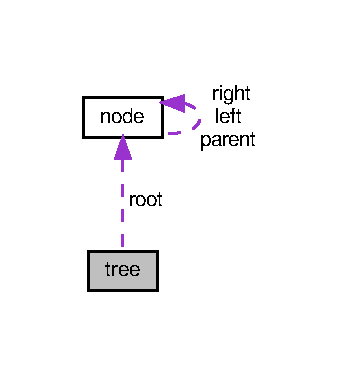
\includegraphics[width=164pt]{classtree__coll__graph}
\end{center}
\end{figure}
\subsection*{Public Member Functions}
\begin{DoxyCompactItemize}
\item 
\hyperlink{classtree_a943d10650f183701ae0414689c9b9ee8}{tree} (vector$<$ int $>$ \&, int n)
\item 
\hyperlink{classtree_a529a530e3787fdaee02ed65cbf1f17ff}{tree} (int n, bool balanced)
\item 
void \hyperlink{classtree_a48edff6ad24225010aa16b36182185d4}{Start} ()
\end{DoxyCompactItemize}
\subsection*{Private Member Functions}
\begin{DoxyCompactItemize}
\item 
void \hyperlink{classtree_a5aa82979670b726692fdf9d0df4248de}{Gen\+B\+ST} (vector$<$ int $>$ \&, int, int, int)
\item 
int \hyperlink{classtree_ac07199db0ed26e80db1ec481bcba7380}{find\+Height} (\hyperlink{structnode}{node} $\ast$N)
\item 
void \hyperlink{classtree_a4dc5cf9375c65041ac594c810072be50}{iniz} (vector$<$ int $>$ \&, int n)
\item 
void \hyperlink{classtree_a09613a8cf3f28dfa51dfd06ceeb90fa0}{draw\+Tree} (int cx, int cy, \hyperlink{structnode}{node} $\ast$N)
\end{DoxyCompactItemize}
\subsection*{Private Attributes}
\begin{DoxyCompactItemize}
\item 
\hyperlink{structnode}{node} $\ast$ \hyperlink{classtree_ad397d4906e47149b98f769b3e81473ee}{root}
\end{DoxyCompactItemize}


\subsection{Constructor \& Destructor Documentation}
\mbox{\Hypertarget{classtree_a943d10650f183701ae0414689c9b9ee8}\label{classtree_a943d10650f183701ae0414689c9b9ee8}} 
\index{tree@{tree}!tree@{tree}}
\index{tree@{tree}!tree@{tree}}
\subsubsection{\texorpdfstring{tree()}{tree()}\hspace{0.1cm}{\footnotesize\ttfamily [1/2]}}
{\footnotesize\ttfamily tree\+::tree (\begin{DoxyParamCaption}\item[{vector$<$ int $>$ \&}]{input,  }\item[{int}]{n }\end{DoxyParamCaption})}

tree constructor which will take the number of nodes n and the array which has the data of each node

tree constructor which takes an input array of n nodes and converts it into a B\+ST \mbox{\Hypertarget{classtree_a529a530e3787fdaee02ed65cbf1f17ff}\label{classtree_a529a530e3787fdaee02ed65cbf1f17ff}} 
\index{tree@{tree}!tree@{tree}}
\index{tree@{tree}!tree@{tree}}
\subsubsection{\texorpdfstring{tree()}{tree()}\hspace{0.1cm}{\footnotesize\ttfamily [2/2]}}
{\footnotesize\ttfamily tree\+::tree (\begin{DoxyParamCaption}\item[{int}]{n,  }\item[{bool}]{balanced }\end{DoxyParamCaption})}

tree constructor which will take the number of nodes n and a boolean value which tells if the tree to be generated is balanced or not

tree constructor which will take the number of nodes n and a boolean dataue which tells if the tree to be generated is balanced or not 

\subsection{Member Function Documentation}
\mbox{\Hypertarget{classtree_a09613a8cf3f28dfa51dfd06ceeb90fa0}\label{classtree_a09613a8cf3f28dfa51dfd06ceeb90fa0}} 
\index{tree@{tree}!draw\+Tree@{draw\+Tree}}
\index{draw\+Tree@{draw\+Tree}!tree@{tree}}
\subsubsection{\texorpdfstring{draw\+Tree()}{drawTree()}}
{\footnotesize\ttfamily void tree\+::draw\+Tree (\begin{DoxyParamCaption}\item[{int}]{cx = {\ttfamily 0},  }\item[{int}]{cy = {\ttfamily 0},  }\item[{\hyperlink{structnode}{node} $\ast$}]{N = {\ttfamily NULL} }\end{DoxyParamCaption})\hspace{0.3cm}{\ttfamily [private]}}

Draws the Binary tree recursively one child at a time. This function takes in the values of x and y of the parent node and draws the daughter node as well as the line connecting it with the parent node The function does this recursively for each child of the node No parameters need to be passed when calling it

Draws the Binary tree recursively one child at a time. This function takes in the values of x and y of the parent node and draws the daughter node as well as the line connecting it with the parent node. \mbox{\Hypertarget{classtree_ac07199db0ed26e80db1ec481bcba7380}\label{classtree_ac07199db0ed26e80db1ec481bcba7380}} 
\index{tree@{tree}!find\+Height@{find\+Height}}
\index{find\+Height@{find\+Height}!tree@{tree}}
\subsubsection{\texorpdfstring{find\+Height()}{findHeight()}}
{\footnotesize\ttfamily int tree\+::find\+Height (\begin{DoxyParamCaption}\item[{\hyperlink{structnode}{node} $\ast$}]{N = {\ttfamily NULL} }\end{DoxyParamCaption})\hspace{0.3cm}{\ttfamily [private]}}

Finds the height of the tree \mbox{\Hypertarget{classtree_a5aa82979670b726692fdf9d0df4248de}\label{classtree_a5aa82979670b726692fdf9d0df4248de}} 
\index{tree@{tree}!Gen\+B\+ST@{Gen\+B\+ST}}
\index{Gen\+B\+ST@{Gen\+B\+ST}!tree@{tree}}
\subsubsection{\texorpdfstring{Gen\+B\+S\+T()}{GenBST()}}
{\footnotesize\ttfamily void tree\+::\+Gen\+B\+ST (\begin{DoxyParamCaption}\item[{vector$<$ int $>$ \&}]{a,  }\item[{int}]{start,  }\item[{int}]{finish,  }\item[{int}]{beg = {\ttfamily 0} }\end{DoxyParamCaption})\hspace{0.3cm}{\ttfamily [private]}}

Array to Balanced Bianary tree; \mbox{\Hypertarget{classtree_a4dc5cf9375c65041ac594c810072be50}\label{classtree_a4dc5cf9375c65041ac594c810072be50}} 
\index{tree@{tree}!iniz@{iniz}}
\index{iniz@{iniz}!tree@{tree}}
\subsubsection{\texorpdfstring{iniz()}{iniz()}}
{\footnotesize\ttfamily void tree\+::iniz (\begin{DoxyParamCaption}\item[{vector$<$ int $>$ \&}]{input,  }\item[{int}]{n }\end{DoxyParamCaption})\hspace{0.3cm}{\ttfamily [private]}}

Generates a B\+ST from a given input array It is used by constructor

This is an private function which generates a B\+ST from a given input array It is used by constructor calls \mbox{\Hypertarget{classtree_a48edff6ad24225010aa16b36182185d4}\label{classtree_a48edff6ad24225010aa16b36182185d4}} 
\index{tree@{tree}!Start@{Start}}
\index{Start@{Start}!tree@{tree}}
\subsubsection{\texorpdfstring{Start()}{Start()}}
{\footnotesize\ttfamily void tree\+::\+Start (\begin{DoxyParamCaption}\item[{void}]{ }\end{DoxyParamCaption})}

This function sets up the initial conditions and calls the functions to implement \textquotesingle{}TR\textquotesingle{} algorithm and draws the tree

This function sets up the initial conditions and calls the functions to implement \textquotesingle{}TR\textquotesingle{} algorithm and draws the tree. 

\subsection{Member Data Documentation}
\mbox{\Hypertarget{classtree_ad397d4906e47149b98f769b3e81473ee}\label{classtree_ad397d4906e47149b98f769b3e81473ee}} 
\index{tree@{tree}!root@{root}}
\index{root@{root}!tree@{tree}}
\subsubsection{\texorpdfstring{root}{root}}
{\footnotesize\ttfamily \hyperlink{structnode}{node}$\ast$ tree\+::root\hspace{0.3cm}{\ttfamily [private]}}

Points to the root of the tree. 

The documentation for this class was generated from the following files\+:\begin{DoxyCompactItemize}
\item 
Computer\+Graphics\+Project/\+Computer\+Graphics\+Project/\hyperlink{tree_8h}{tree.\+h}\item 
Computer\+Graphics\+Project/\+Computer\+Graphics\+Project/\hyperlink{tree_8cpp}{tree.\+cpp}\end{DoxyCompactItemize}

\chapter{File Documentation}
\hypertarget{_circle_8cpp}{}\section{Computer\+Graphics\+Project/\+Computer\+Graphics\+Project/\+Circle.cpp File Reference}
\label{_circle_8cpp}\index{Computer\+Graphics\+Project/\+Computer\+Graphics\+Project/\+Circle.\+cpp@{Computer\+Graphics\+Project/\+Computer\+Graphics\+Project/\+Circle.\+cpp}}
{\ttfamily \#include $<$G\+L/glew.\+h$>$}\newline
{\ttfamily \#include \char`\"{}Circle.\+h\char`\"{}}\newline
{\ttfamily \#include $<$G\+L/freeglut.\+h$>$}\newline
Include dependency graph for Circle.\+cpp\+:
\nopagebreak
\begin{figure}[H]
\begin{center}
\leavevmode
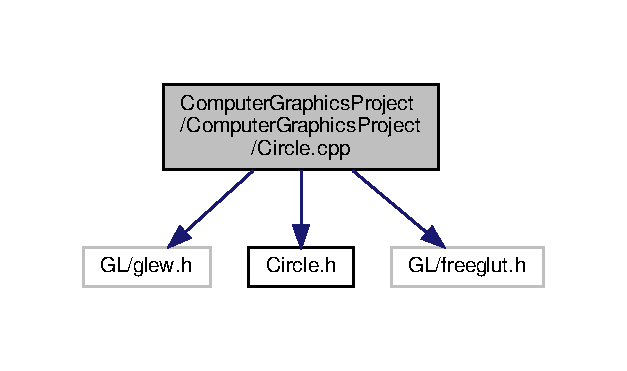
\includegraphics[width=301pt]{_circle_8cpp__incl}
\end{center}
\end{figure}
\subsection*{Functions}
\begin{DoxyCompactItemize}
\item 
void \hyperlink{_circle_8cpp_a5308e773395d45dcc2e6941cc99e9931}{Plot\+\_\+\+Px} (G\+Lint x, G\+Lint y, double r=0, double g=0, double b=0)
\end{DoxyCompactItemize}


\subsection{Function Documentation}
\mbox{\Hypertarget{_circle_8cpp_a5308e773395d45dcc2e6941cc99e9931}\label{_circle_8cpp_a5308e773395d45dcc2e6941cc99e9931}} 
\index{Circle.\+cpp@{Circle.\+cpp}!Plot\+\_\+\+Px@{Plot\+\_\+\+Px}}
\index{Plot\+\_\+\+Px@{Plot\+\_\+\+Px}!Circle.\+cpp@{Circle.\+cpp}}
\subsubsection{\texorpdfstring{Plot\+\_\+\+Px()}{Plot\_Px()}}
{\footnotesize\ttfamily void Plot\+\_\+\+Px (\begin{DoxyParamCaption}\item[{G\+Lint}]{x,  }\item[{G\+Lint}]{y,  }\item[{double}]{r = {\ttfamily 0},  }\item[{double}]{g = {\ttfamily 0},  }\item[{double}]{b = {\ttfamily 0} }\end{DoxyParamCaption})}


\hypertarget{_circle_8h}{}\section{Computer\+Graphics\+Project/\+Computer\+Graphics\+Project/\+Circle.h File Reference}
\label{_circle_8h}\index{Computer\+Graphics\+Project/\+Computer\+Graphics\+Project/\+Circle.\+h@{Computer\+Graphics\+Project/\+Computer\+Graphics\+Project/\+Circle.\+h}}
This graph shows which files directly or indirectly include this file\+:
\nopagebreak
\begin{figure}[H]
\begin{center}
\leavevmode
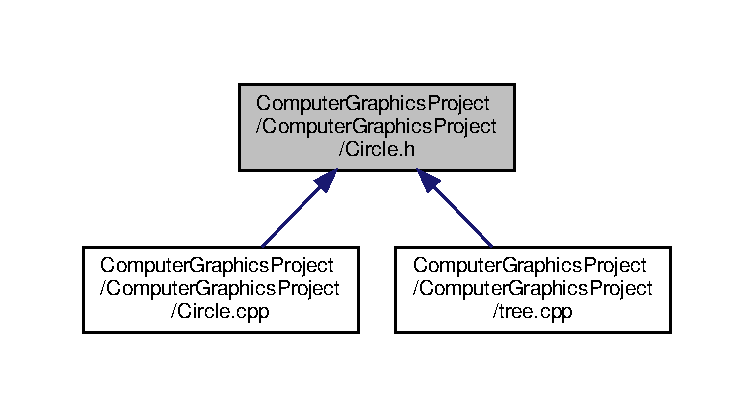
\includegraphics[width=350pt]{_circle_8h__dep__incl}
\end{center}
\end{figure}
\subsection*{Classes}
\begin{DoxyCompactItemize}
\item 
class \hyperlink{classcircle}{circle}
\end{DoxyCompactItemize}

\hypertarget{_line_8cpp}{}\section{Computer\+Graphics\+Project/\+Computer\+Graphics\+Project/\+Line.cpp File Reference}
\label{_line_8cpp}\index{Computer\+Graphics\+Project/\+Computer\+Graphics\+Project/\+Line.\+cpp@{Computer\+Graphics\+Project/\+Computer\+Graphics\+Project/\+Line.\+cpp}}
{\ttfamily \#include \char`\"{}Line.\+h\char`\"{}}\newline
{\ttfamily \#include $<$math.\+h$>$}\newline
{\ttfamily \#include $<$gl/glew.\+h$>$}\newline
{\ttfamily \#include $<$G\+L/\+G\+L.\+h$>$}\newline
Include dependency graph for Line.\+cpp\+:
\nopagebreak
\begin{figure}[H]
\begin{center}
\leavevmode
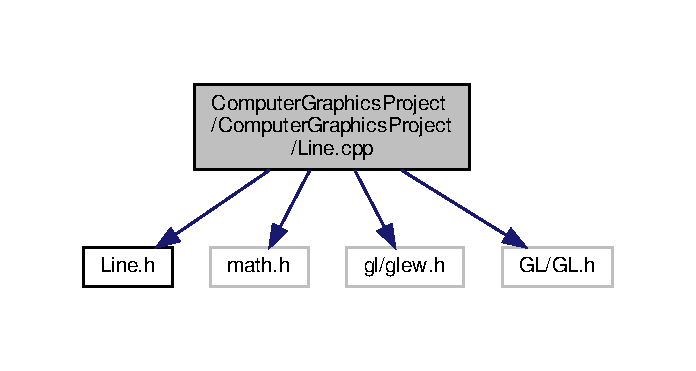
\includegraphics[width=334pt]{_line_8cpp__incl}
\end{center}
\end{figure}

\hypertarget{_line_8h}{}\section{Computer\+Graphics\+Project/\+Computer\+Graphics\+Project/\+Line.h File Reference}
\label{_line_8h}\index{Computer\+Graphics\+Project/\+Computer\+Graphics\+Project/\+Line.\+h@{Computer\+Graphics\+Project/\+Computer\+Graphics\+Project/\+Line.\+h}}
This graph shows which files directly or indirectly include this file\+:
\nopagebreak
\begin{figure}[H]
\begin{center}
\leavevmode
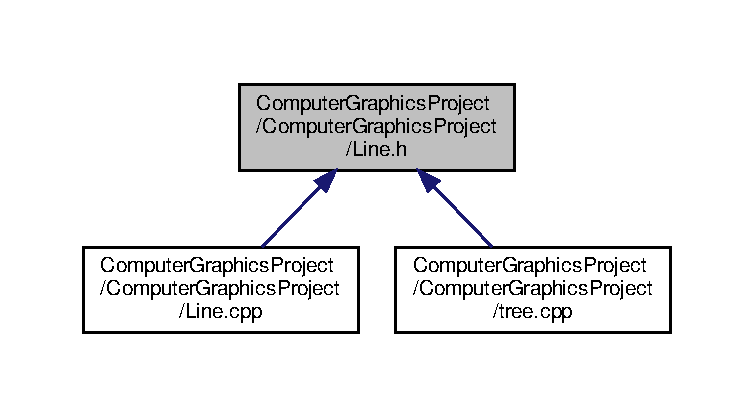
\includegraphics[width=350pt]{_line_8h__dep__incl}
\end{center}
\end{figure}
\subsection*{Classes}
\begin{DoxyCompactItemize}
\item 
class \hyperlink{classline}{line}
\end{DoxyCompactItemize}

\hypertarget{main_8cpp}{}\section{Computer\+Graphics\+Project/\+Computer\+Graphics\+Project/main.cpp File Reference}
\label{main_8cpp}\index{Computer\+Graphics\+Project/\+Computer\+Graphics\+Project/main.\+cpp@{Computer\+Graphics\+Project/\+Computer\+Graphics\+Project/main.\+cpp}}
{\ttfamily \#include $<$iostream$>$}\newline
{\ttfamily \#include \char`\"{}tree.\+h\char`\"{}}\newline
{\ttfamily \#include $<$math.\+h$>$}\newline
{\ttfamily \#include $<$gl/glew.\+h$>$}\newline
{\ttfamily \#include $<$G\+L/\+G\+L.\+h$>$}\newline
{\ttfamily \#include $<$vector$>$}\newline
{\ttfamily \#include $<$G\+L/freeglut.\+h$>$}\newline
Include dependency graph for main.\+cpp\+:
\nopagebreak
\begin{figure}[H]
\begin{center}
\leavevmode
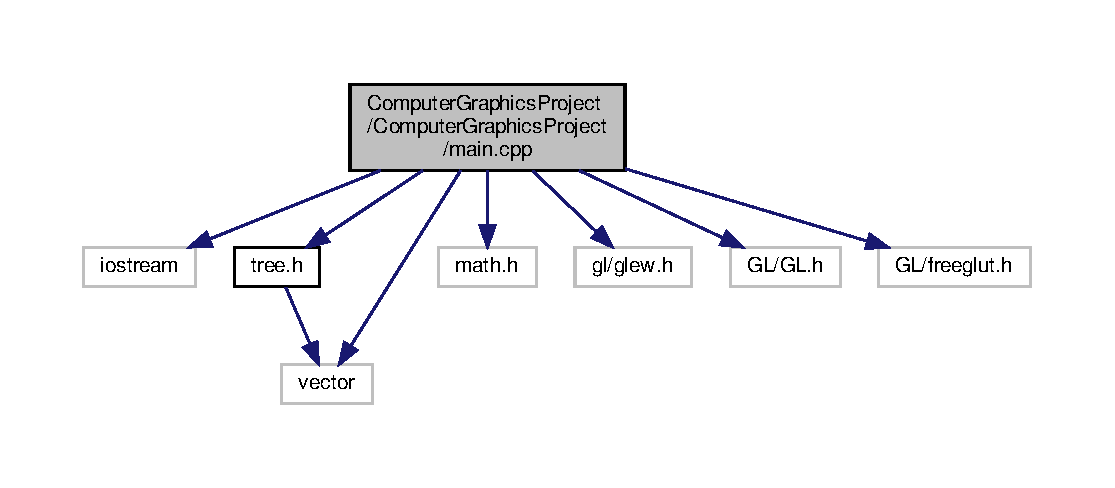
\includegraphics[width=350pt]{main_8cpp__incl}
\end{center}
\end{figure}
\subsection*{Functions}
\begin{DoxyCompactItemize}
\item 
void \hyperlink{main_8cpp_a02fd73d861ef2e4aabb38c0c9ff82947}{init} ()
\item 
void \hyperlink{main_8cpp_ac88040080eff31ce13de964b86e1cfa6}{draw\+\_\+tree} (void)
\item 
int \hyperlink{main_8cpp_a3c04138a5bfe5d72780bb7e82a18e627}{main} (int argc, char $\ast$$\ast$argv)
\end{DoxyCompactItemize}
\subsection*{Variables}
\begin{DoxyCompactItemize}
\item 
\hyperlink{classtree}{tree} $\ast$ \hyperlink{main_8cpp_aee3ab5f8e61528be92ff53e823e93bc3}{t}
\end{DoxyCompactItemize}


\subsection{Function Documentation}
\mbox{\Hypertarget{main_8cpp_ac88040080eff31ce13de964b86e1cfa6}\label{main_8cpp_ac88040080eff31ce13de964b86e1cfa6}} 
\index{main.\+cpp@{main.\+cpp}!draw\+\_\+tree@{draw\+\_\+tree}}
\index{draw\+\_\+tree@{draw\+\_\+tree}!main.\+cpp@{main.\+cpp}}
\subsubsection{\texorpdfstring{draw\+\_\+tree()}{draw\_tree()}}
{\footnotesize\ttfamily void draw\+\_\+tree (\begin{DoxyParamCaption}\item[{void}]{ }\end{DoxyParamCaption})}

\mbox{\Hypertarget{main_8cpp_a02fd73d861ef2e4aabb38c0c9ff82947}\label{main_8cpp_a02fd73d861ef2e4aabb38c0c9ff82947}} 
\index{main.\+cpp@{main.\+cpp}!init@{init}}
\index{init@{init}!main.\+cpp@{main.\+cpp}}
\subsubsection{\texorpdfstring{init()}{init()}}
{\footnotesize\ttfamily void init (\begin{DoxyParamCaption}{ }\end{DoxyParamCaption})}

\mbox{\Hypertarget{main_8cpp_a3c04138a5bfe5d72780bb7e82a18e627}\label{main_8cpp_a3c04138a5bfe5d72780bb7e82a18e627}} 
\index{main.\+cpp@{main.\+cpp}!main@{main}}
\index{main@{main}!main.\+cpp@{main.\+cpp}}
\subsubsection{\texorpdfstring{main()}{main()}}
{\footnotesize\ttfamily int main (\begin{DoxyParamCaption}\item[{int}]{argc,  }\item[{char $\ast$$\ast$}]{argv }\end{DoxyParamCaption})}



\subsection{Variable Documentation}
\mbox{\Hypertarget{main_8cpp_aee3ab5f8e61528be92ff53e823e93bc3}\label{main_8cpp_aee3ab5f8e61528be92ff53e823e93bc3}} 
\index{main.\+cpp@{main.\+cpp}!t@{t}}
\index{t@{t}!main.\+cpp@{main.\+cpp}}
\subsubsection{\texorpdfstring{t}{t}}
{\footnotesize\ttfamily \hyperlink{classtree}{tree}$\ast$ t}


\hypertarget{tree_8cpp}{}\section{Computer\+Graphics\+Project/\+Computer\+Graphics\+Project/tree.cpp File Reference}
\label{tree_8cpp}\index{Computer\+Graphics\+Project/\+Computer\+Graphics\+Project/tree.\+cpp@{Computer\+Graphics\+Project/\+Computer\+Graphics\+Project/tree.\+cpp}}
{\ttfamily \#include \char`\"{}tree.\+h\char`\"{}}\newline
{\ttfamily \#include \char`\"{}Line.\+h\char`\"{}}\newline
{\ttfamily \#include \char`\"{}Circle.\+h\char`\"{}}\newline
{\ttfamily \#include $<$math.\+h$>$}\newline
{\ttfamily \#include $<$gl/glew.\+h$>$}\newline
{\ttfamily \#include $<$G\+L/\+G\+L.\+h$>$}\newline
{\ttfamily \#include $<$cstdlib$>$}\newline
{\ttfamily \#include $<$G\+L/freeglut.\+h$>$}\newline
{\ttfamily \#include $<$iostream$>$}\newline
{\ttfamily \#include $<$time.\+h$>$}\newline
{\ttfamily \#include $<$vector$>$}\newline
Include dependency graph for tree.\+cpp\+:
\nopagebreak
\begin{figure}[H]
\begin{center}
\leavevmode
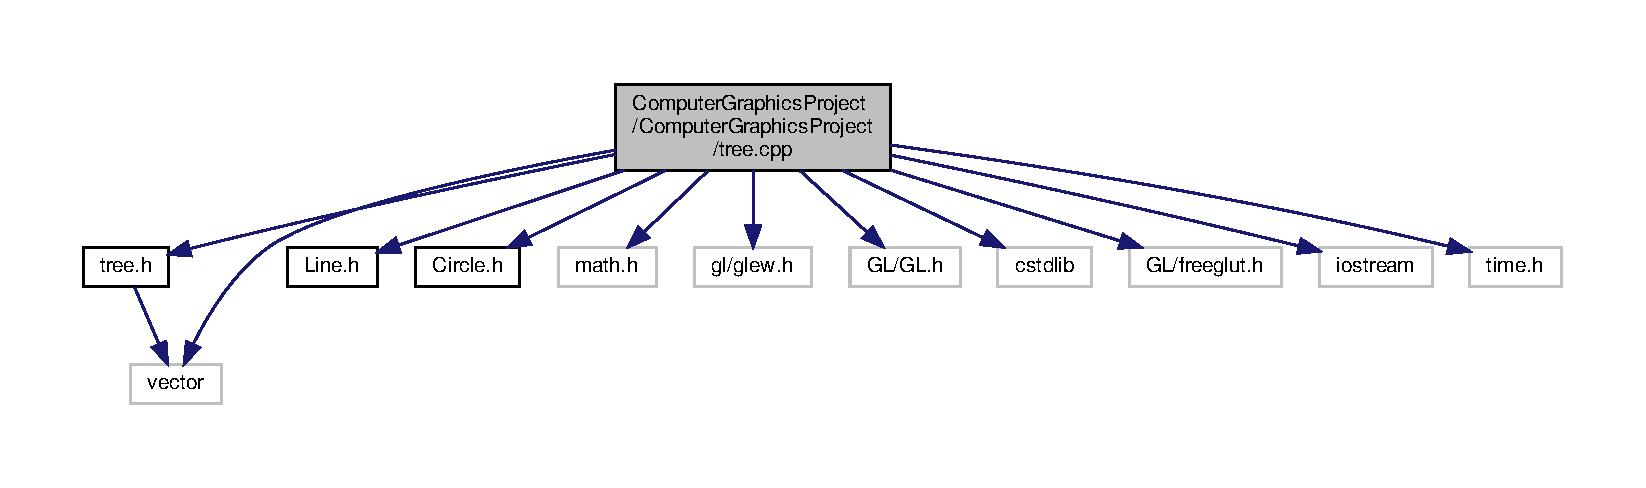
\includegraphics[width=350pt]{tree_8cpp__incl}
\end{center}
\end{figure}
\subsection*{Macros}
\begin{DoxyCompactItemize}
\item 
\#define \hyperlink{tree_8cpp_af0b629d98f0b3df05f708edbf99c0728}{rr}~10
\item 
\#define \hyperlink{tree_8cpp_a66cb98cee4ec0167b1ed423368bbb86d}{M\+I\+N\+S\+EP}~50
\item 
\#define \hyperlink{tree_8cpp_af8dc443bbe421682422f11ce80d943e8}{Y\+S\+C\+A\+LE}~30
\end{DoxyCompactItemize}
\subsection*{Functions}
\begin{DoxyCompactItemize}
\item 
int \hyperlink{tree_8cpp_af082905f7eac6d03e92015146bbc1925}{max} (int a, int b)
\item 
int \hyperlink{tree_8cpp_a673a4c7055d7c5d2d4f1e736b436340f}{Random\+\_\+num} (int l, int u)
\item 
void \hyperlink{tree_8cpp_a30a73c71774dd933ba586eb4e5934e21}{setup\+\_\+tdr} (\hyperlink{structnode}{node} $\ast$root, int level, \hyperlink{structextreme}{extreme} \&rightmost, \hyperlink{structextreme}{extreme} \&leftmost)
\item 
void \hyperlink{tree_8cpp_abbdc20412b9c1b9342d701e8f5f9257c}{traverse} (\hyperlink{structnode}{node} $\ast$root, int col)
\end{DoxyCompactItemize}


\subsection{Macro Definition Documentation}
\mbox{\Hypertarget{tree_8cpp_a66cb98cee4ec0167b1ed423368bbb86d}\label{tree_8cpp_a66cb98cee4ec0167b1ed423368bbb86d}} 
\index{tree.\+cpp@{tree.\+cpp}!M\+I\+N\+S\+EP@{M\+I\+N\+S\+EP}}
\index{M\+I\+N\+S\+EP@{M\+I\+N\+S\+EP}!tree.\+cpp@{tree.\+cpp}}
\subsubsection{\texorpdfstring{M\+I\+N\+S\+EP}{MINSEP}}
{\footnotesize\ttfamily \#define M\+I\+N\+S\+EP~50}

\mbox{\Hypertarget{tree_8cpp_af0b629d98f0b3df05f708edbf99c0728}\label{tree_8cpp_af0b629d98f0b3df05f708edbf99c0728}} 
\index{tree.\+cpp@{tree.\+cpp}!rr@{rr}}
\index{rr@{rr}!tree.\+cpp@{tree.\+cpp}}
\subsubsection{\texorpdfstring{rr}{rr}}
{\footnotesize\ttfamily \#define rr~10}

\mbox{\Hypertarget{tree_8cpp_af8dc443bbe421682422f11ce80d943e8}\label{tree_8cpp_af8dc443bbe421682422f11ce80d943e8}} 
\index{tree.\+cpp@{tree.\+cpp}!Y\+S\+C\+A\+LE@{Y\+S\+C\+A\+LE}}
\index{Y\+S\+C\+A\+LE@{Y\+S\+C\+A\+LE}!tree.\+cpp@{tree.\+cpp}}
\subsubsection{\texorpdfstring{Y\+S\+C\+A\+LE}{YSCALE}}
{\footnotesize\ttfamily \#define Y\+S\+C\+A\+LE~30}



\subsection{Function Documentation}
\mbox{\Hypertarget{tree_8cpp_af082905f7eac6d03e92015146bbc1925}\label{tree_8cpp_af082905f7eac6d03e92015146bbc1925}} 
\index{tree.\+cpp@{tree.\+cpp}!max@{max}}
\index{max@{max}!tree.\+cpp@{tree.\+cpp}}
\subsubsection{\texorpdfstring{max()}{max()}}
{\footnotesize\ttfamily int max (\begin{DoxyParamCaption}\item[{int}]{a,  }\item[{int}]{b }\end{DoxyParamCaption})}

Returns the grater number of the two \mbox{\Hypertarget{tree_8cpp_a673a4c7055d7c5d2d4f1e736b436340f}\label{tree_8cpp_a673a4c7055d7c5d2d4f1e736b436340f}} 
\index{tree.\+cpp@{tree.\+cpp}!Random\+\_\+num@{Random\+\_\+num}}
\index{Random\+\_\+num@{Random\+\_\+num}!tree.\+cpp@{tree.\+cpp}}
\subsubsection{\texorpdfstring{Random\+\_\+num()}{Random\_num()}}
{\footnotesize\ttfamily int Random\+\_\+num (\begin{DoxyParamCaption}\item[{int}]{l,  }\item[{int}]{u }\end{DoxyParamCaption})}

Returns a random number from l to u inclusive \mbox{\Hypertarget{tree_8cpp_a30a73c71774dd933ba586eb4e5934e21}\label{tree_8cpp_a30a73c71774dd933ba586eb4e5934e21}} 
\index{tree.\+cpp@{tree.\+cpp}!setup\+\_\+tdr@{setup\+\_\+tdr}}
\index{setup\+\_\+tdr@{setup\+\_\+tdr}!tree.\+cpp@{tree.\+cpp}}
\subsubsection{\texorpdfstring{setup\+\_\+tdr()}{setup\_tdr()}}
{\footnotesize\ttfamily void setup\+\_\+tdr (\begin{DoxyParamCaption}\item[{\hyperlink{structnode}{node} $\ast$}]{root,  }\item[{int}]{level,  }\item[{\hyperlink{structextreme}{extreme} \&}]{rightmost,  }\item[{\hyperlink{structextreme}{extreme} \&}]{leftmost }\end{DoxyParamCaption})}

This function finds and evaluates all offsets for drawing the tree which are stored int the node defined in node class \mbox{\Hypertarget{tree_8cpp_abbdc20412b9c1b9342d701e8f5f9257c}\label{tree_8cpp_abbdc20412b9c1b9342d701e8f5f9257c}} 
\index{tree.\+cpp@{tree.\+cpp}!traverse@{traverse}}
\index{traverse@{traverse}!tree.\+cpp@{tree.\+cpp}}
\subsubsection{\texorpdfstring{traverse()}{traverse()}}
{\footnotesize\ttfamily void traverse (\begin{DoxyParamCaption}\item[{\hyperlink{structnode}{node} $\ast$}]{root,  }\item[{int}]{col }\end{DoxyParamCaption})}

This procedures forms the pre-\/order traversal of the tree converting the relative coordinates to absolute coordinates 
\hypertarget{tree_8h}{}\section{Computer\+Graphics\+Project/\+Computer\+Graphics\+Project/tree.h File Reference}
\label{tree_8h}\index{Computer\+Graphics\+Project/\+Computer\+Graphics\+Project/tree.\+h@{Computer\+Graphics\+Project/\+Computer\+Graphics\+Project/tree.\+h}}
{\ttfamily \#include $<$vector$>$}\newline
Include dependency graph for tree.\+h\+:
\nopagebreak
\begin{figure}[H]
\begin{center}
\leavevmode
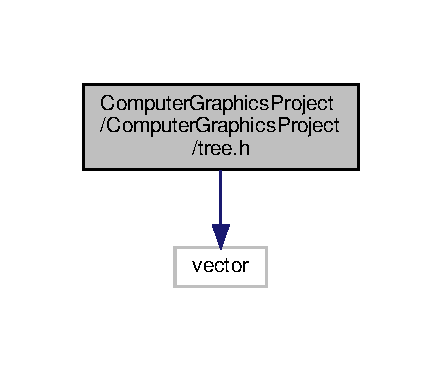
\includegraphics[width=212pt]{tree_8h__incl}
\end{center}
\end{figure}
This graph shows which files directly or indirectly include this file\+:
\nopagebreak
\begin{figure}[H]
\begin{center}
\leavevmode
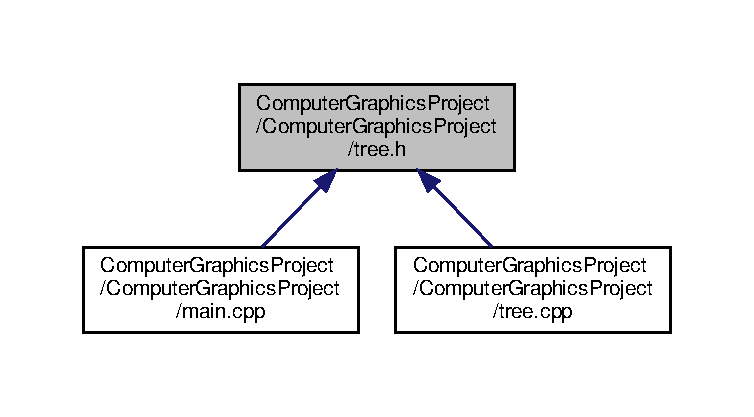
\includegraphics[width=350pt]{tree_8h__dep__incl}
\end{center}
\end{figure}
\subsection*{Classes}
\begin{DoxyCompactItemize}
\item 
struct \hyperlink{structnode}{node}
\item 
struct \hyperlink{structextreme}{extreme}
\item 
class \hyperlink{classtree}{tree}
\end{DoxyCompactItemize}
\subsection*{Typedefs}
\begin{DoxyCompactItemize}
\item 
typedef struct \hyperlink{structnode}{node} \hyperlink{tree_8h_af4aeda155dbe167f1c1cf38cb65bf324}{node}
\item 
typedef struct \hyperlink{structextreme}{extreme} \hyperlink{tree_8h_aca506b23b36c98c5e97eed4d29e79900}{extreme}
\end{DoxyCompactItemize}


\subsection{Typedef Documentation}
\mbox{\Hypertarget{tree_8h_aca506b23b36c98c5e97eed4d29e79900}\label{tree_8h_aca506b23b36c98c5e97eed4d29e79900}} 
\index{tree.\+h@{tree.\+h}!extreme@{extreme}}
\index{extreme@{extreme}!tree.\+h@{tree.\+h}}
\subsubsection{\texorpdfstring{extreme}{extreme}}
{\footnotesize\ttfamily typedef struct \hyperlink{structextreme}{extreme} \hyperlink{structextreme}{extreme}}

\mbox{\Hypertarget{tree_8h_af4aeda155dbe167f1c1cf38cb65bf324}\label{tree_8h_af4aeda155dbe167f1c1cf38cb65bf324}} 
\index{tree.\+h@{tree.\+h}!node@{node}}
\index{node@{node}!tree.\+h@{tree.\+h}}
\subsubsection{\texorpdfstring{node}{node}}
{\footnotesize\ttfamily typedef struct \hyperlink{structnode}{node} \hyperlink{structnode}{node}}


%--- End generated contents ---

% Index
\backmatter
\newpage
\phantomsection
\clearemptydoublepage
\addcontentsline{toc}{chapter}{Index}
\printindex

\end{document}
